% =========================================================
% Chapter: Methodology I — Hybrid Visual Deepfake Detection
% Purpose:
% - Describe the video-only (Phase I) detection pipeline end-to-end
% - Focus on what each module does (spatial encoder, temporal model, attention, classifier)
% - Provide practical, implementation-oriented details for reproducibility
% Navigation:
% - Sections: Problem framing, architecture (with subsections), data/preprocessing, training protocol, ablations
% Tips:
% - Keep math minimal; emphasize design rationale and practical choices
% =========================================================
\chapter{Methodology I: Hybrid Visual Deepfake Detection}
\label{ch:method-visual}

This chapter details the Phase I system: a video-only hybrid deep learning architecture that integrates spatial feature extraction, bidirectional temporal modeling, and sequence-level attention to detect visual deepfakes. The design addresses limitations of single-frame CNNs by explicitly modeling temporal dynamics and enabling the classifier to focus on salient temporal segments indicative of manipulation.

% High-level description of the task; notation here is only to set context (kept minimal)
\section{Problem Formulation}
We frame deepfake detection as a binary classification task on short video clips of fixed length. Each clip is labeled as authentic (real) or manipulated (fake). The model outputs a confidence score for the manipulated class and is trained with a standard binary classification objective, without presenting formal equations here for readability.

% Overview of the Phase I pipeline and how components connect (frame encoder -> temporal model -> attention -> head)
\section{Proposed Architecture}
The architecture consists of three main stages: (i) frame-level spatial encoding via ResNet50, (ii) sequence modeling via Bidirectional GRUs (Bi-GRUs), and (iii) Multi-Head Attention (MHA) to enhance focus on temporally salient features, followed by a classification head.

% Frame-level spatial encoder: extracts robust per-frame features; pretrained weights improve generalization
\subsection{Spatial Feature Extraction (ResNet50)}
Each frame is processed by a ResNet50 backbone (pretrained on ImageNet-1K) with its final classification layer removed to extract a per-frame embedding (2048-D for ResNet50). This produces a sequence of per-frame feature vectors that captures spatial cues such as blending artifacts, boundary inconsistencies, and subtle textural anomalies \cite{rossler2019faceforensics,afchar2018mesonet}.

% Temporal modeling: Bi-GRU captures forward/backward temporal context to expose inconsistencies in motion/behavior
\subsection{Bidirectional Temporal Modeling (Bi-GRU)}
To capture temporal dependencies indicative of manipulation (e.g., blink patterns, motion jitter), the spatial embeddings are fed to a two-layer Bidirectional GRU. Bidirectionality enables the model to leverage both past and future context at each time step, improving detection of temporally extended anomalies \cite{guera2018deepfake,dey2017gru}.

% Temporal self-attention: reweights time steps to emphasize salient segments and suppress irrelevant variation
\subsection{Multi-Head Attention over Temporal Features}
Attention emphasizes salient temporal regions and aggregates sequence information for classification. A multi-head temporal self-attention layer reweights the time steps to highlight short segments that are most indicative of manipulation, while suppressing irrelevant variations. The final sequence representation is obtained by pooling the attention-weighted features and projecting them for classification, without presenting formal attention equations.

% Shallow feed-forward head: maps the aggregated sequence representation to a calibrated probability
\subsection{Classification Head}
The final classification head consists of fully connected layers that map the fused representation to a binary decision (real or fake). Consistent with the accompanying paper, layer normalization is used to stabilize learning dynamics and a GELU activation is applied before the final prediction layer.
The overall workflow of the Phase~I architecture is shown in Figure~\ref{fig:phase1-arch}.

\begin{figure}[!htbp]
\centering
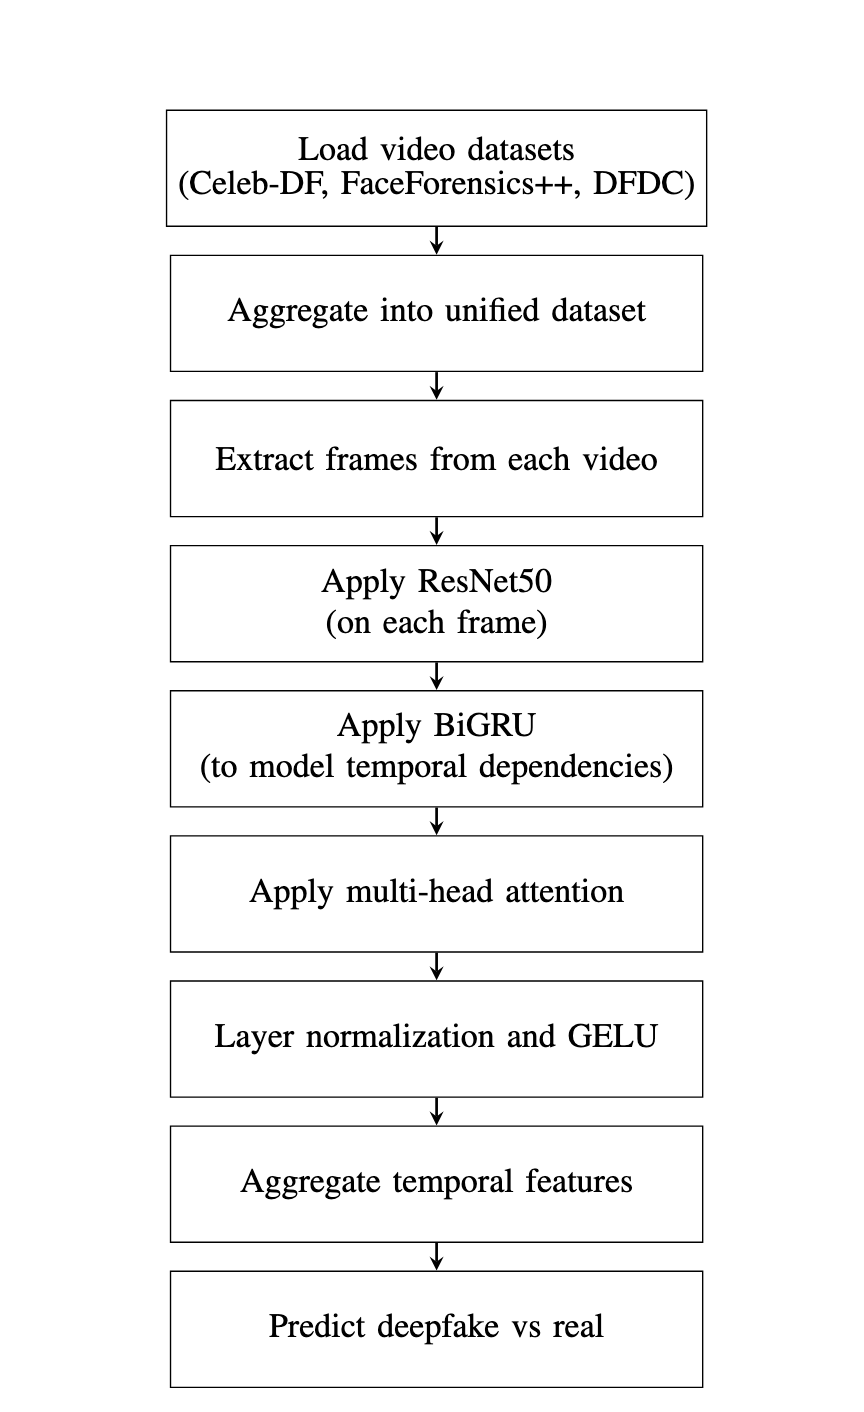
\includegraphics[width=0.95\linewidth]{diagrams/paper1_architecture.png}
\caption{Workflow of the Proposed Hybrid Deep Learning Architecture for Deepfake Detection.}
\label{fig:phase1-arch}
\end{figure}

% Datasets and preprocessing: how videos are sampled, faces cropped/aligned, normalized, and augmented
\section{Dataset Description and Preprocessing}
% Benchmarks included for aggregated training to reduce dataset bias and improve cross-dataset generalization
\subsection{Benchmarks}
Training leverages an aggregated corpus to promote generalization and reduce dataset-specific bias:
\begin{itemize}
    \item \textbf{FaceForensics++ (FF++)} \cite{rossler2019faceforensics}: 1000 source videos with multiple manipulation methods (DeepFakes, Face2Face, FaceSwap, NeuralTextures).
    \item \textbf{Celeb-DF} \cite{li2020celebdf}: 590 originals and 5{,}639 high-quality deepfakes with reduced visible artifacts.
    \item \textbf{Deepfake Detection Challenge (DFDC)} \cite{dolhansky2020dfdc}: Large-scale dataset (>100k clips) with diverse subjects, methods, and augmentations.
\end{itemize}
Combining these benchmarks exposes the model to varied artifacts and content distributions \cite{gong2024survey}.

% End-to-end preprocessing steps; apply the same policy consistently across datasets for fair training
\subsection{Preprocessing Pipeline}
\begin{itemize}
    \item \textbf{Frame Extraction and Face Cropping:} Videos are split into individual frames, and a face detection algorithm is used to crop the face region.
    \item \textbf{Resizing and Normalization:} Cropped frames are resized to 112x112 pixels and normalized using the ImageNet mean and standard deviation.
    \item \textbf{Frame Sampling Strategy:} A fixed frame sampling strategy of 10 fps is used for consistency.
\end{itemize}

% Augmentation goals: improve robustness, simulate real-world degradations; apply transforms consistently across time
\subsection{Data Augmentation}
To improve robustness and mitigate overfitting, temporally consistent augmentations are applied across frames \cite{mubarak2023survey}:
\begin{itemize}
    \item \textbf{Geometric:} Random horizontal flips, rotations, scaling, and translations.
    \item \textbf{Photometric:} Brightness, contrast, saturation jitter.
    \item \textbf{Degradations:} Blur, noise, and compression-like artifacts.
\end{itemize}

% Practical training details: optimizer, schedules, regularization, precision, and early stopping
\section{Training Protocol}
The model is trained on the aggregated benchmark using the preprocessing and augmentation strategy described above. In line with the accompanying paper, the experimental analysis emphasizes the contribution of dataset aggregation, consistent augmentation, and the interaction among the ResNet50 backbone, Bi-GRU temporal modeling, and Multi-Head Attention.

\subsection{Implementation Focus}
ResNet50 serves as the spatial encoder, the Bi-GRU captures temporal inconsistencies across frame sequences, and the Multi-Head Attention block emphasizes the most informative temporal regions before binary classification. The reported study evaluates this full configuration against simplified variants that remove attention, remove recurrent modeling, or replace the backbone.

% Ablations isolate the contribution of each component (attention, temporal modeling, backbone, data aggregation)
\section{Ablation Study Design}
To quantify the contribution of each component, the following ablations are evaluated on held-out test sets:
\begin{enumerate}[leftmargin=*]
    \item \textbf{No Attention:} Remove MHA and replace with mean temporal pooling over Bi-GRU outputs.
    \item \textbf{No Temporal Modeling:} Remove Bi-GRU and perform temporal average pooling directly on frame embeddings.
    \item \textbf{Backbone Variant:} Replace ResNet50 with a light CNN to assess sensitivity to spatial encoder quality.
    \item \textbf{Single-Dataset Training:} Train on each dataset individually to assess cross-dataset generalization gaps.
\end{enumerate}

% Pipeline diagram: visual overview of Phase I data flow from frames to final decision
% Recap of Phase I methodology and how it sets up the experiments in Chapter~\ref{ch:experiments}
\section{Summary}
The hybrid architecture marries strong spatial encodings with explicit temporal modeling and attention-based sequence aggregation. By training on a diverse aggregation of benchmarks with realistic augmentations, the system targets generalization to unseen manipulations and robustness under practical degradations. Results for this phase, including comparative baselines and ablations, are presented in Chapter~\ref{ch:experiments} alongside multimodal results from Phase II.
However, Phase~I focuses exclusively on visual cues. In practice, hybrid forgeries can manipulate only one modality (e.g., forged video with genuine audio or vice versa). To address this vulnerability, Phase~II extends detection to the audio–visual setting and explicitly models synchrony between visemes and phonemes.

% Local labels for cross-references from other chapters
\label{sec:methodology-visual}
